\documentclass{article}

\usepackage{hyperref}
\hypersetup{
	colorlinks=true,
	linkcolor=blue,
	filecolor=magenta,      
	urlcolor=cyan
}
\usepackage[american]{circuitikz}
\usepackage{siunitx}
\usepackage{amsmath}

\begin{document}
	This document explains from Bohr model of atoms to how a PN junction work, and focuses on building a mental model that helps understanding how electrons move in devices like diodes, MOSFETs and BJTs.
	\section{Bohr Model and periodic table}
		Useful Resource : \href{https://www.youtube.com/watch?v=OCTAQaubQ4o&ab_channel=WayneBreslyn%28Dr.B.%29}{Atomic Structure for Silicon Video}, \href{https://pubchem.ncbi.nlm.nih.gov/periodic-table/}{Periodic Table}\\\\
		Quick review that Silicon's atomic number is 14, which means a neutral atom of silicon has 14 electrons. The horizontal count by rows on the periodic table means the number of electrons in each shell.
		\begin{center}
			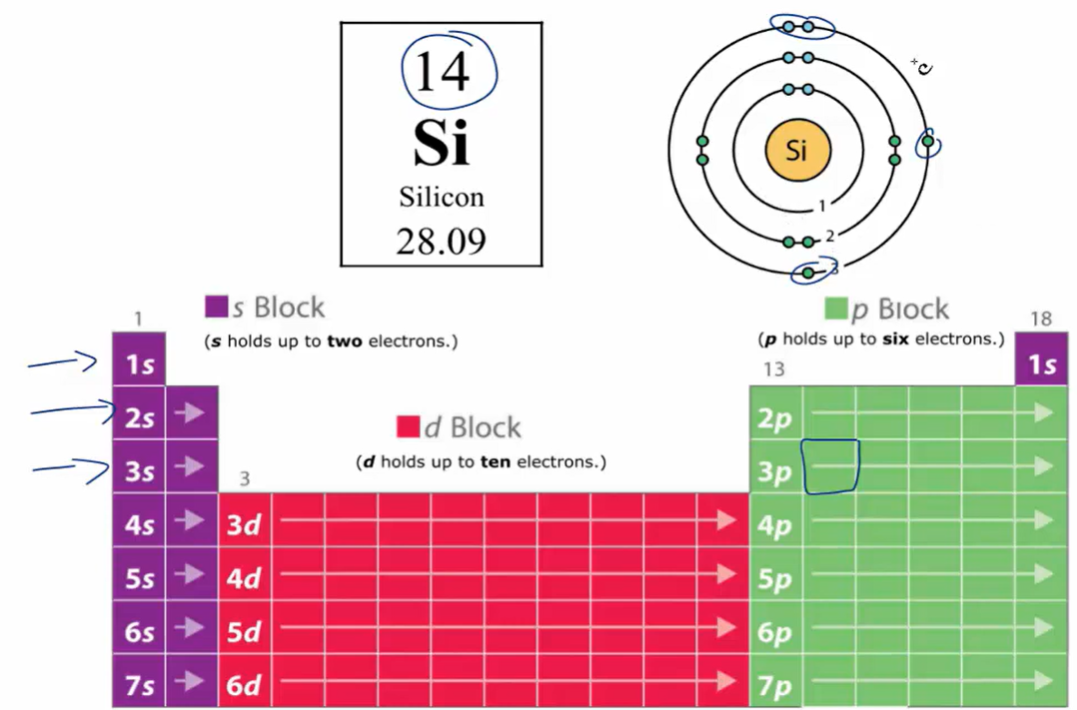
\includegraphics[width=\textwidth]{img/si_element.png}
		\end{center}
		We can see that silicon has 4 electrons in the valence shell(outer most shell), since the count from left to right on the third row is 4.
		\begin{center}
			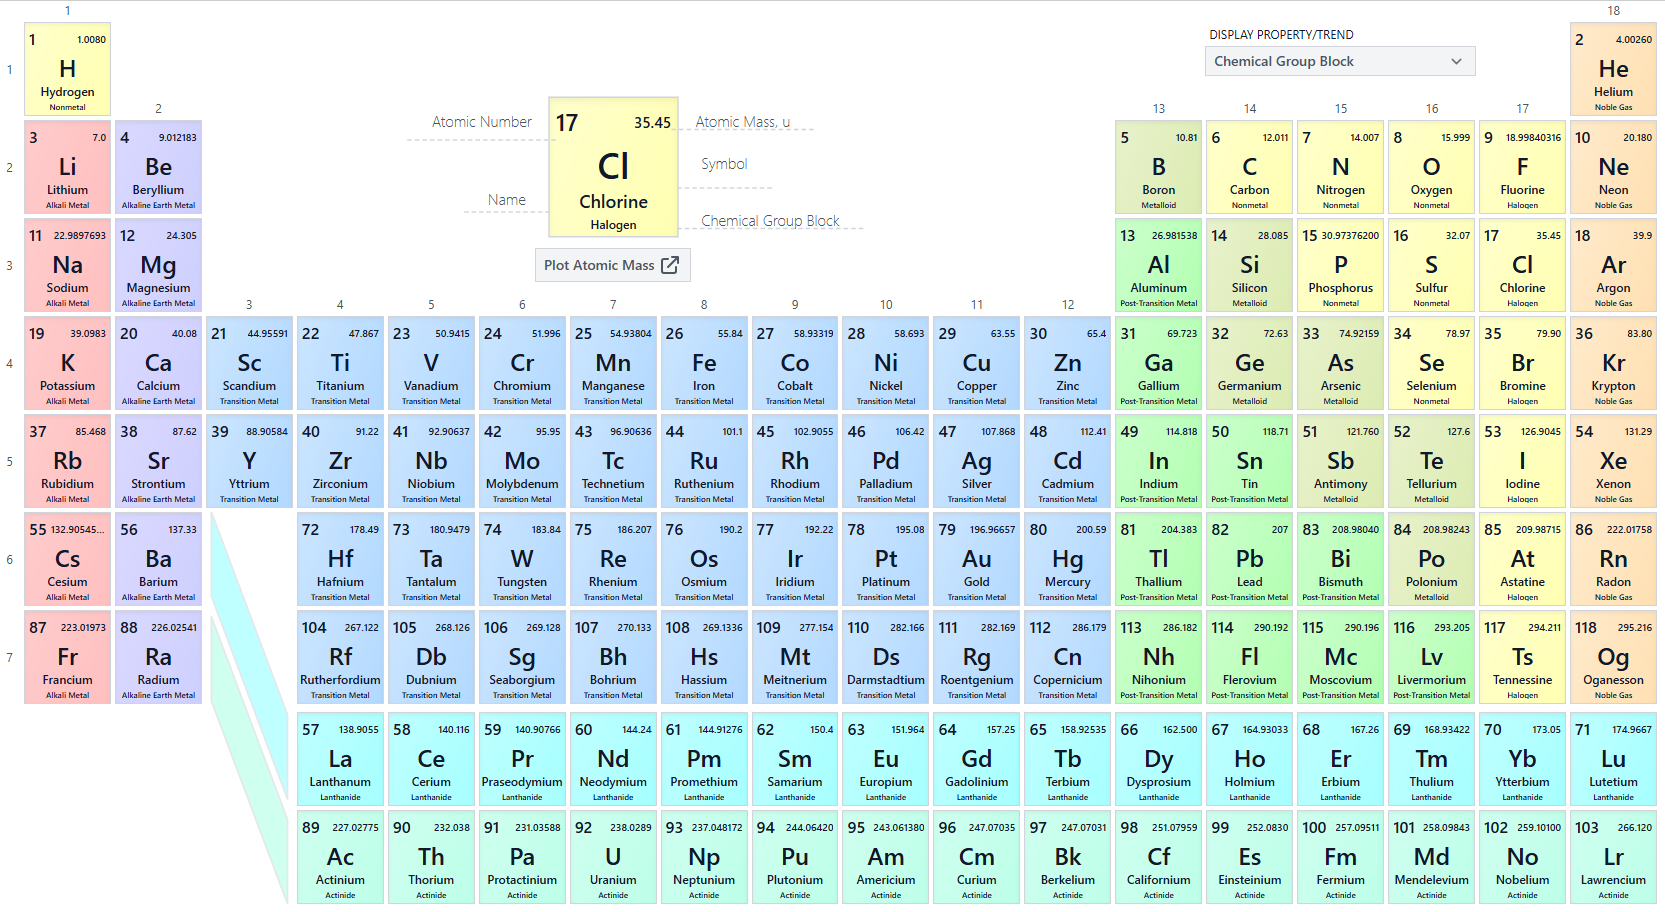
\includegraphics[width=\textwidth]{img/periodic_table.png}
		\end{center}
	\section{Doping}
		Useful Resource : \href{https://www.youtube.com/watch?v=ErcH_OuCaNY&list=PLfYdTiQCV_p7sDswtLZKK43BWOd2mTmHC&index=3&ab_channel=CircuitBread}{Intrinsic and Extrinsic semiconductors}
	 	$Si^+$ means that a silicon atom lost an electron, so only 3 electrons in the valence shell, Vice versa for $Si^{-}$.\\
	 	Doping is inserting different neutral atoms into a silicon crystal. A crystal structure is when atoms are nicely lined up, repeated arrangement of atoms, just like the picture below.
	 	\begin{center}
	 		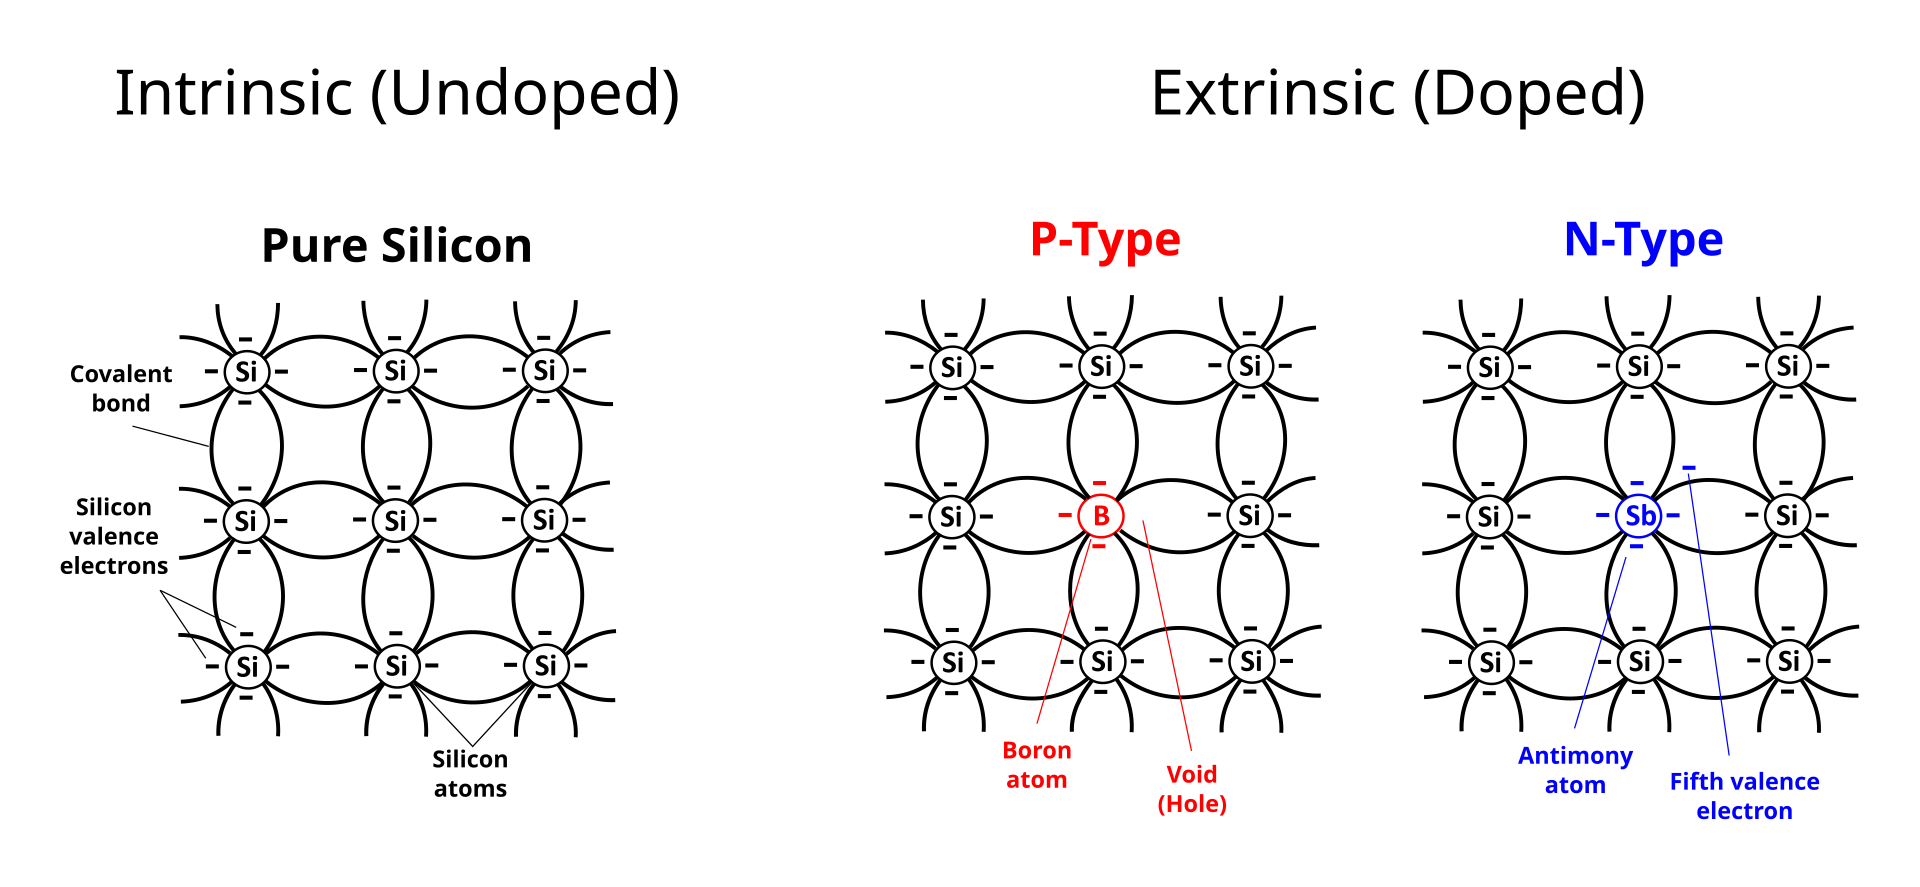
\includegraphics[width=\textwidth]{img/si_doping.png}
	 	\end{center}
	 	From the periodic table horizontal element count, we can see that silicon's valence shell is missing 4 electrons, and it just happens to have 4 free electrons in the valence shell as well. So in a pure silicon crystalline structure the Si atoms will share the 4 electrons. The specifics of covalent bond will not be omitted here. Some common element for doping includes\\\\
	 	Acceptors, valence shell have 1 less(than 4) electron, aka trivalent impurities. This forms P-type extrinsic semiconductor:
	 	\begin{itemize}
	 		\item Boron(B, 5)
	 		\item Aluminum(Al, 13)
	 		\item Gallium(Ga, 31)
	 	\end{itemize}
	 	Donors, valence shell have 1 more(than 4) electron, aka pentavalent impurities. This forms N-type extrinsic semiconductor:
	 	\begin{itemize}
	 		\item Phosphorus(P, 15)
	 		\item Arsenic(As, 33)
	 		\item Antimony(Sb, 51)
	 	\end{itemize}
	 	We can see the positions of these elements relative to silicon's position on the periodic table. Acceptors to the left, donors to the left.
	 \section{Electron \& Hole Movement and Conventional Current}
	 	Remember that conventional current is the opposite direction as the electron moving direction.\\
	 	In P-type semiconductor, holes are the majority current carrier whereas in N-type semiconductor, electrons are the majority current carrier. In both types, the conventional current flow and electron flow directions are same. See the movement of electron in the following images:
	 	\begin{center}
	 		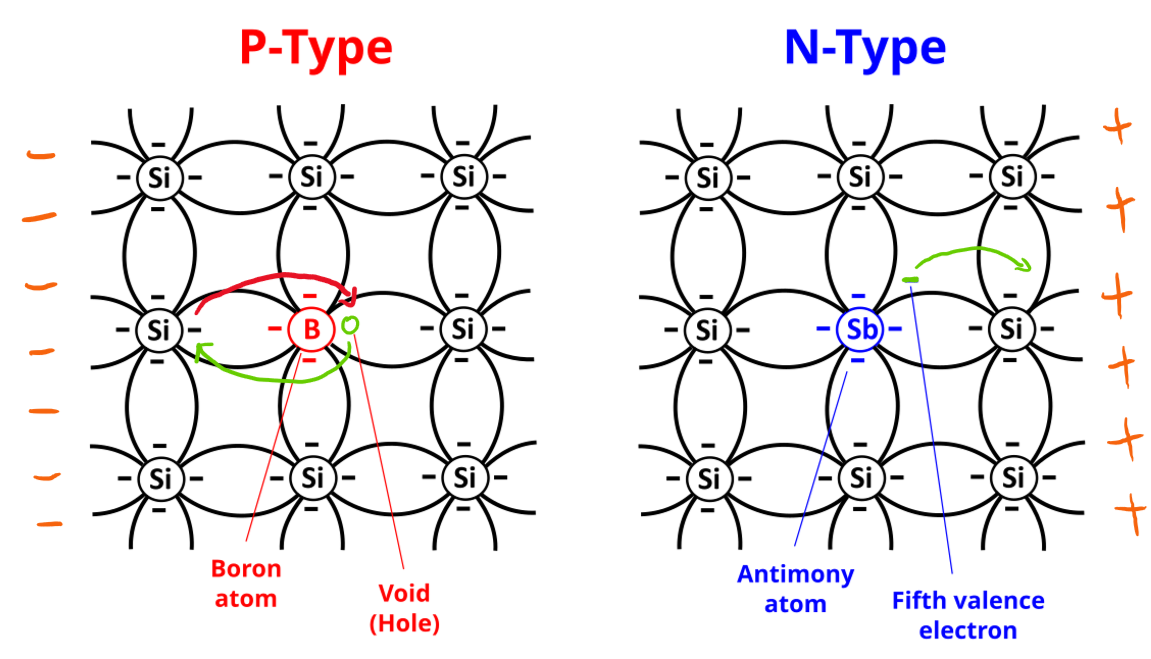
\includegraphics[width=\textwidth]{img/current_flow_1.png}
	 		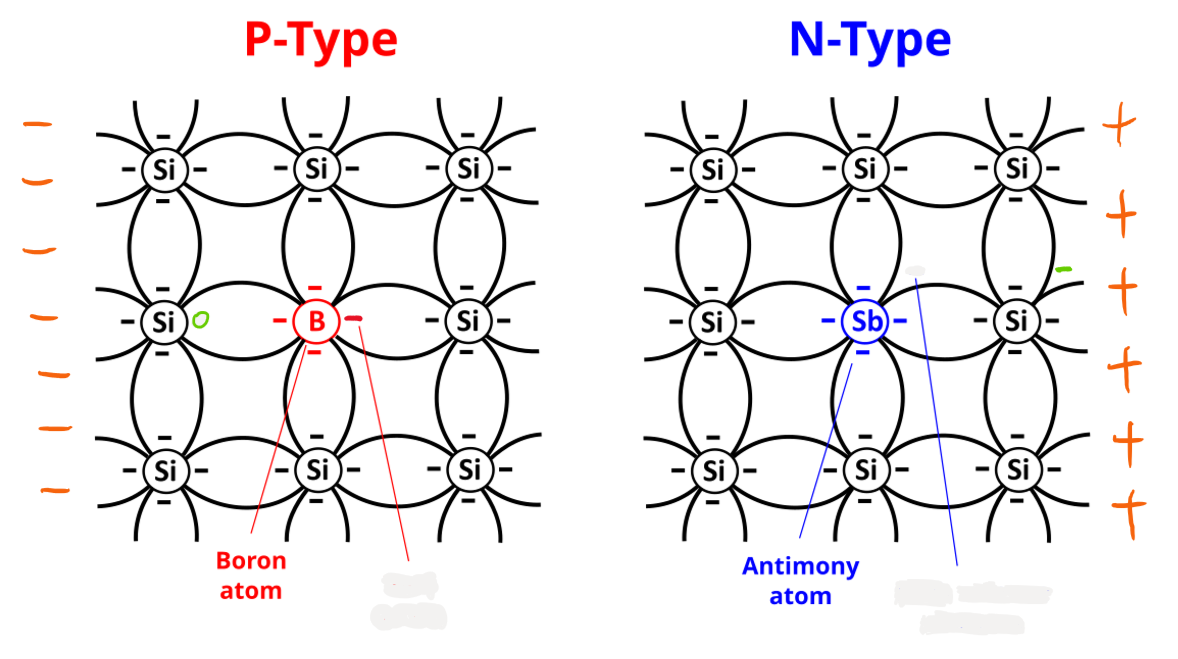
\includegraphics[width=\textwidth]{img/current_flow_2.png}
	 	\end{center}
	 	The \textcolor{orange}{orange label} are just indicators of electric field, showing that free electron flow is from left to right in both semiconductors. This shows that \textbf{conventional current in both semiconductors are from right to left}. Holes move in the same direction as conventional current.\\
	 	\\
	 	This is why the source terminal in N and P type MOSFETs are called source because they are the source of charge carriers
	 	\begin{circuitikz}
	 		%% draw p and nmos and indicate conventional current, electron and hole direction
	 	\end{circuitikz}
	 	
	 	
		
		
\end{document}